\appendix
\chapter{Code source}
\begin{figure}[H]
	\centering
	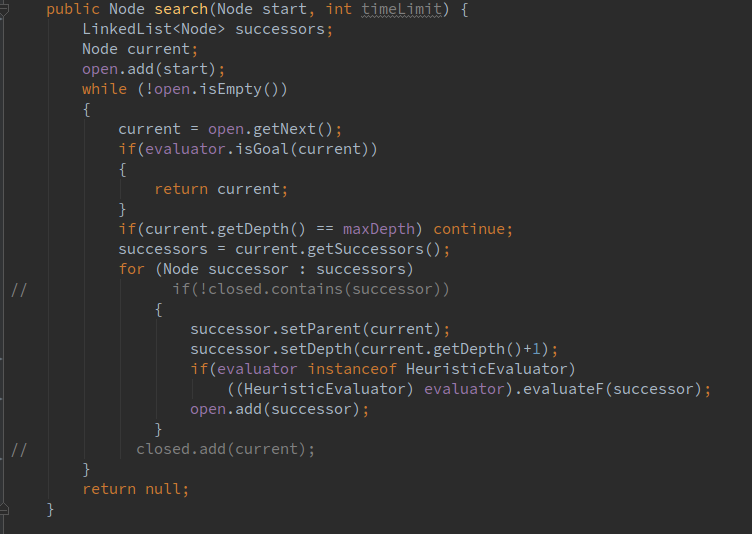
\includegraphics[width=\textwidth]{images/imgs/graphSearch.png}
	\caption{Algorithme de recherche principal}
\end{figure}

\begin{figure}[H]
	\centering
	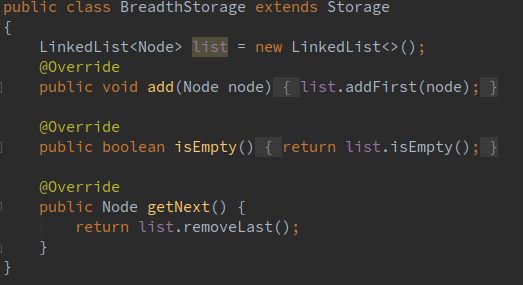
\includegraphics[width=\textwidth]{images/imgs/BFSstorage.png}
	\caption{Gestion de open en largeur d'abord}
\end{figure}

\begin{figure}[H]
	\centering
	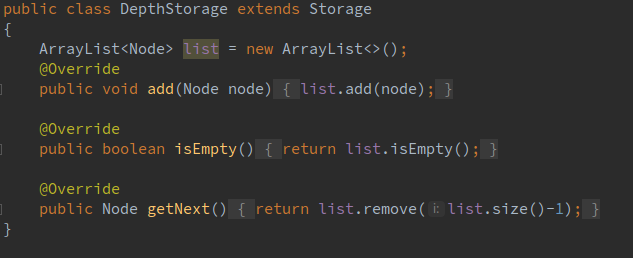
\includegraphics[width=\textwidth]{images/imgs/DFSStorage.png}
	\caption{Gestion de open par profondeur d'abord}
\end{figure}

\begin{figure}[H]
	\centering
	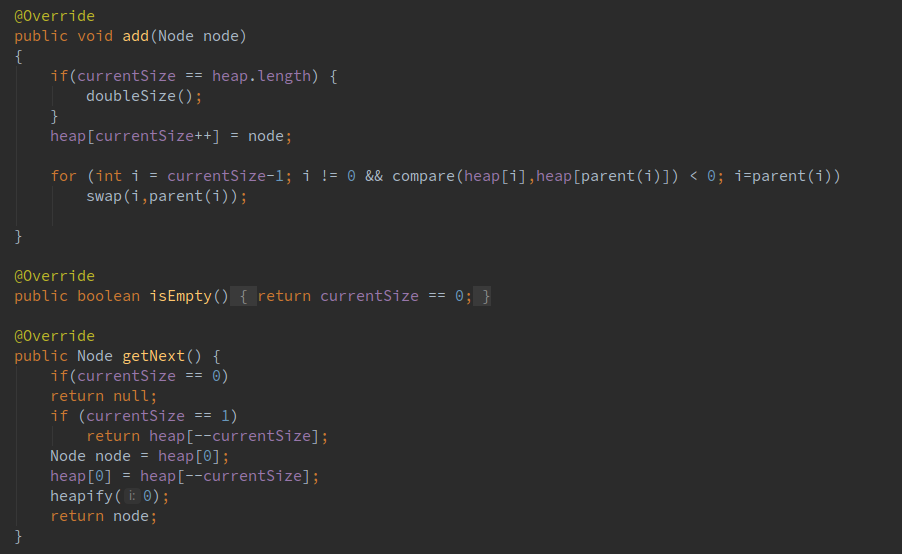
\includegraphics[width=\textwidth]{images/imgs/heapStorage.png}
	\caption{Gestion de open en tant que tas}
\end{figure}

\begin{figure}[H]
	\centering
	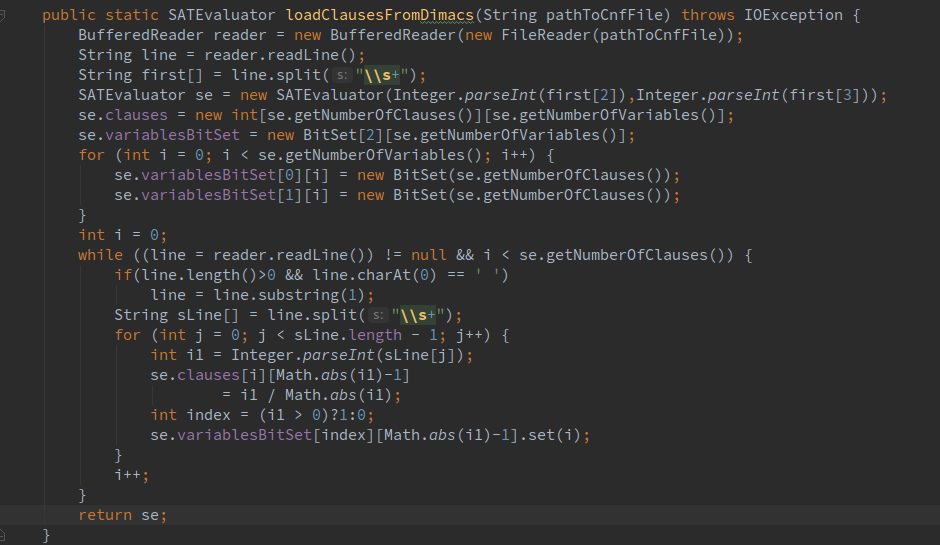
\includegraphics[width=\textwidth]{images/imgs/loadFromDimacs.png}
	\caption{Chargement de l'instance depuis le fichier benchmark}
\end{figure}

\begin{figure}[H]
	\centering
	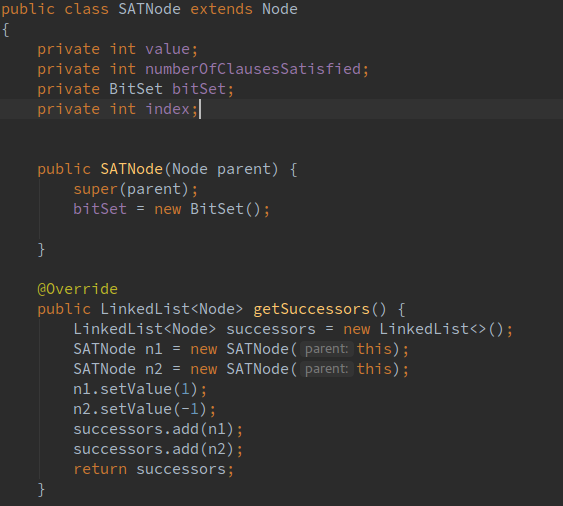
\includegraphics[width=\textwidth]{images/imgs/nodeStruct.png}
	\caption{Structure d'un noeud dans l'arborescence}
\end{figure}